\documentclass{article}
\usepackage{mathtools,natbib}
\title{Ice fabric development with a new fabric evolution model}
\author{Michael Hay}
\begin{document}
\maketitle

\begin{abstract}
Ice crystal orientatation fabric has a strong influence on ice flow due to the plastic anisotropy of ice. Anisotropy can also induce folding and boudinage of layers, which complicates paleoclimate interpretation. In addition, crystal fabric evolution coupled to ice deformation can exhibit hysteresis, which is ignored in current treatments. This can be a source of tilted cone fabrics \citep{throstur2002}, which can induce vertical shear strain in response to horizontal simple shear. The evolution of crystal fabric is driven by strain-induced grain rotation, as well as recrystallization. Most fabric evolution models ignore much of the physical processes involved, or are valid only for highly parameterized fabrics. In this paper, we outline a new fabric model which treats a variety of processes affecting fabric development, and is suitable for inclusion in flow models. The model is validated against thin-section data from the WAIS divide core. In addition, numerical experiments investigating the differential thinning of layers possessing different initial conditions is mainvestigating the differential thinning of layers possessing different initial conditions is madee. 
\end{abstract}

\section{Introduction}
An individual ice crystal has an anisotropic creep response, deforming most easily in shear parallel to the crystal basal plane. Plastic deformation of an ice polycrystal depends on the orientations of its constituent grains \citep{azuma94}. A polycrystal that is initially isotropic will develop a lattice-preffered orientation in response to applied strain, thus causing it to have a bulk anisotropic response. The development of a preferred orientation is guided primarily by intracrystalline slip. Due to interference between grains, there is a tendency for the c-axis to rotate away from extensional axes. In addition to rotation, recrystallization effects both grain size and orientation distribution. Near the melting point, migration recrystallization allows the nucleation of new, strain-free grains. These new grains rapidly grow at the expense of older grains with high strain energy \citep{duval1995}. Polygonization is another recrystallization process in which dislocations of a highy strained grain arrange into a subgrain boundary, eventually producing two grains as the misalignment increases \citep{alley97}. Although the grains typically are only misaligned by a few degrees, this does have the effect of preventing the orientation distribution function from attaining sharp maxima.

In order to model fabric development, a homogenization scheme must be used in order to relate the macroscopic stress and strain rate experienced by the polycrystal to the state experienced by individual grains. The two possible endmembers are the Taylor-Bishop-Hill (homogeneous strain) \citep{taylor} and the Sachs (homogeneous stress) \citep{sachs} assumptions. For many materials such as metals with several active slip systems, homogeneous strain turns out to be a good assumption. It has the advantage of maintaining compatibility in between grains, in assuming that hard-oriented grains recieve correspondingly more stress in order to produce the same strain as soft grains. For ice, in which basal dislocation glide is by far the easiest slip system, homogeneous stress is a better assumption \citep{thorsteinsson2002nni}. The actual situation is somewhere in the middle, with softer-oriented grains receiving more strain. Grain compatibility is maintained compatibility through intercrystalline slip and shear on basal and non-basal slip systems. \citet{molinari} developed the viscoplastic self-consistent homogenization (VPSC) model. Each individual grain is represented as an inclusion in a homogeneous equivalent medium representative of the bulk polycrystal properties. This is a compromise between the homogeneous stress and homogeneous strain assumptions. The VPSC model has been used for ice by several investigators (e.g. \citet{gillet2005}). \citet{azuma96} used a conceptually similar scheme in which stress over the polycrystal is partitioned by the resolved shear stress on the basal plane of each individual crystal. \citet{thorsteinsson2002nni} takes a different approach using the assumption of a polycrystal with cube-like topology, with each grain having six neighboring grains. The strain on each individual crystal is adjusted by a softness parameter depending on the resolved shear stress on the neighboring grains. A grain surrounded by hard-oriented grains becomes softer from the nearest neighbor interaction, whereas one surrounded by soft grains becomes harder.

Anisotropic ice flow models usually do not have a fabric evolution component (e.g. \citet{pettit2007}) or employ a highly parameterized orientation distribution function \citep{gillet2006}. There have been several grain-scale models developed. In this paper, we outline a more general probabilistic fabric evolution model. Instead of examining a continous orientation distribution function, it uses a sample of individual grains to represent a region. Each grain posesses various physical properties such as radius, strain, etc. In addition, each grain has several neighbors grains, with which it interacts. This is somewhat similar to the approach \citet{thorsteinsson2002nni} and \citet{kennedy} took to account for nearest neighbor interactions. However, the previous works assumed each grain has 6 neighbors, whereas this model allows for more or fewer neighbors. The most unique feature is that the model maintains mass balance in the polycrystal. Grains grow only at the expense of neighboring grains, as opposed to assuming a parabolic growth-law. Recrystallization also follows obeys mass balance, with the nucleated grain removing mass from its neighbors. Increases in average grain size can only occur by the disappearance of some grains. It is designed to be incorporated into an anisotropic flow model, as it uses strain rate and vorticity, as opposed to stress, as the model input. 

\section{Grain rotation}
Probably the most important process governing the formation of crystal fabrics is deformation-induced grain rotation. Grain rotation is described using a Jefferys-Type equation \citep{azuma94}:
\[
 \dot{c} = W \cdot c + D \cdot c + c c^T \cdot D \cdot c
\],
where $c$ is the unit vector in the direction of the c-axis, $D$ is the strain rate tensor, and $W$ is the spin tensor. This relates the macroscopic velocity gradient to the change in orientation of each crystal. \citet{gillet2005} instead model the evolution of the second order orientation tensor, $<c \otimes c >$, with an equation derived from Jeffery's equation for a single grain. This has the advantage of only requiring the integration of six independent values. More generally, orientation distribution functions can be written as expansions using orientation distribution tensors $a^{(i)}$ as the basis functions. In this respect, solutions based on orientation tensors terminate this expansion after the $a^{(2)}$ term. By evolving each particle with Jeffery's equation separately, more general fabrics can be handled. 

If deviatoric stress rather than the velocity gradient is supplied, it is possible to calculate the vorticity, and thus the rotation rate, of each grain directly: From the bulk stress, the resolved shear stress of each slip system of individual grains is calculated. From this, shear strain along each slip system, and vorticity can be calculted. The rotation rate is then given by the dot product of the grain vorticity tensor and its c-axis normal vector. This method, however, is difficult to integrate with flow models, as it depends on stress, rather than strain. It is difficult to partition a predetermined bulk strain rate between individual grains and their slip systems.

\section{Grain radius evolution}
To track the rheological properties of a polycrystal, it is necessary to know the volume of each grain. Grain boundaries migrate in order to minimize energy from dislocation density, grain boundary energy, and other factors. The assumptions on the interactions between grains are the following: Three-dimensional grains have a surface area proportional to $r^2$ and a volume proportional to $r^3$, where $r_i$ is the radius of a sphere with the same volume. Assuming a constant scaled shape between grains, then a polycrystal of grains $\{g_i}$ with volume $V=\sum v_i$ where $v_i$ is the volume of grain $i$, has surface area $S=\sum s_i$. For any three-dimensional shape, $\frac{\alpha}{r} v_i =  s_i$, for some constant $\alpha$. Thus, $S=\beta \sum r_i^2$, for some constant $\beta$.

Let $g^{\star}$ be an arbitrary interior grain. This grain has neighbors $g_1,...,g_m$, with radii $r_i$. $g$ has a surface area $T$. The surface $g^{\star}$ shares with neighbor $n_i$ is $S_i$, with surface area $s_i$. Now, assume that $s_i$ is proportional the the surface area of grain $g_i$, or equivalently, $s_i=\alpha r_i^2$.

Now, examine the interface between $g^{\star}$ and $n_i$. Due to grain growth, recrystallization, or other processes, this moves with velocity $v_i$ outwardly normal to the surface. Thus, taken over all neighboring grains, $\frac{dV^{\star}}{dt}=\sum_{i}s_i v_i$. Therefore, if a velocity between two grains can be determined, then this provides a means of determining grain size evolution based on the properties of a grain and its neighbors.

To implement this for a polycrystal, the less computationally intensive way is to declare that each grain has several neighbors with which to determine the growth rate. To deal with grains disappearing or nucleating, originally the polycrystal is declared to have a number of grains with zero radius. Nucleated grains simply assign a nonzero radius to a formerly zero radius grain, and consumed grains are assigned a zero radius. 

\section{Grain Growth}
Normal grain growth is induced by a driving force related to the local curvature at the grain surface

From \citet{durand2006}, the grain boundary velocity between two grains due to normal grain growth can be given by

\[\frac{dr_1}{dt} = K \left( \frac{1}{r_1}-\frac{1}{r_2} \right)
\]

where $K$ is an Arrhenius factor dependent on temperature, and $P$. The difficulty in implementing this using the procedure outlined in the previous section is to determine the radius of curvature at the boundary between the two grains. Clearly, the curvature of each grain must be the negative of the other. In addition, taken over the entire boundary, the integral of the curvature over the boundary of the grain must always be $4 \pi$. This means that, for example, the grain having negative curvature must ``make up'' that curvature elsewhere on its boundary. A reasonable way to handle this (which this model takes)  is to take the curvature of the boundary to be the harmonic mean of the curvatures of the two surfaces. This means that the smaller grain will have positive curvature on the boundary, which is a reasonable assumption. 

\section{Recrystallization}
Migration (dynamic) recrystallization is primarily driven by lower strain energy grains consuming higher strain energy grains \citep{duval1995}. At least at larger scales (after the initial nucleation), this reduction in strain energy can be incorporated into the driving force of grain boundary migration. A grain neighboring a more highly strained grain will advance into the highly strained grain. This is due to the more highly strained grain having higher dislocation density. The dislocations are annihilated by the advancing boundary. 

To determine plastic strain, it is necessary to partition the bulk strain rate between grains. First, the bulk polycrystal stress tensor must be determined. In the coordinate system defined by the c-axis, an individual grain possesses a fourth-order viscosity tensor which can be represented as a diagonal $6x6$ matrix in Voigt notation. The viscosity of the bulk polycrystal is then taken to be the volume-weighted average of each grain's viscosity tensor rotated into the macroscopic coordinate system. Then, the bulk stress tensor is found from the product of the viscosity tensor and the strain-rate tensor. Then, the strain rate of individual grains is determined from the bulk stress tensor and the anisotropic viscosity of the individual grain. The model calculates the effective stress on each grain following \citet{azuma96}, which depends on the bulk stress and the orientation of each grain and its neighbors.  


\section{Model Validation}
The model can reproduce characteristic fabrics for a variety of flow situations, such as single maxima, as well as large girdle fabrics. By incorporating recrystallization, double girdle fabrics and small girdles are produced. This is in qualitative agreement with typical ice-core fabrics types. In figure 1, examples are given of several fabric types produced from different flow scenarios. We validated the model by forcing it with data from the WAIS divide ice core, including temperature and a thinning function derived from the WDC06 chronology. This is then compared to thin-section data collected from the core (Donald Voigt, personal communication).

\subsection{Thin Section Data}
The ice-core thin section data consist of 54 thin sections from depths of 140 meters to 3405 meters, and a corresponding age range of 480 years to $67,800$ B.P. There are several hundred grains in each thin section. The thin sections fabrics display oscillitory behavior. In figure 2, the smallest singular value of each sample is plotted. There are large excursions in several places, which are much too large to be explained by sampling error. 

The fabric model itself is conceptually a Lagrangian model tracking a packet of grains as they are advected through the ice sheet over time, whereas each thin section posesses different initial conditions and physical properties. Thus, a this is expected to be a significant source of mismatch between between observed fabric and modeled fabric. The thin section at 140 m already shows significant development of a preferred orientation. This is in line with the results of \citet{diprinzio2005} at Siple Dome, where preffered orientations were observed in the firn as shallow as 22 m. In addition, at the Siple Dome site, recrystallization was found in some layers of shallow, cold ice. A similar process may contribute to the variability observed in the WAIS thin sections.

 In addition to likely spatial inhomogeneities, there is sampling error due to small size of fabric samples. From modeling experiments, \citet{thorsteinsson2002nni} found that a sample size of around 5000 is needed for a small model variance, whereas the thin sections have sample sizes in the hundreds. However, sampling error is not enough to account for the large differences in fabric seen in the core.    

A common method to summarize a fabric with grain orientations $X$ is to calculate eigenvalues and eigenvectors of the matrix formed by $X X'$. This can capture certain general features such as the strength of a single maximum fabric or a girdle fabric. However, it is unable to capture non-linear features of orientation distributions. For our analysis, we summarize fabrics using the ``earth mover distance'' (EMD). The EMD between two point sets $P_1$ and $P_2$, with vectors of associated weights for each point $W_1$ and $W_2$, is given by the minimum work required to move the weights from points on $P_1$ to the points on $P_2$. In this case, we are transforming c-axis normal vectors from one observed fabric to another across the upper hemisphere. The work to move a weight $w$ from a point $x$ to a point $y$ on the upper hemisphere is then given by ${wd}$, where $d$ is the great-circle distance. This measure can detect changes in fabric which are not reflected in the fabric eigenvalues, such as the difference between a double girdle and a diffuse single girdle. In addition, it is a relatively robust measure, with qualitatively similar fabrics producing similar results. To model the "girdleness" and single-maximum strength of a fabric, we measure the EMD between the fabric and a perfect single maximum and a perfect girdle. That is, fabrics with c-axis orientations concentrated at only one point, in the case of a single maximum fabric, or along a plane, in the case of a girdle fabric. The results are shown in figure !!THE FIGURE!!. 



\subsection{Conclusions}


!!FIGURE: Several curves of EMD to girdle and single maxima plotted with different recrystalization probability paramters. Subplot: Schmidt plots of fabrics at different depths.!!


\begin{figure}
\caption{Plot of the modeled smallest  singular value of the modeled fabric versus that of the WAIS thin section data. In the upper part of the core, there is a large girdle from extension in one horizontal axis, tending towards a single maximum as simple shear increases. Corresponding Schmidt plots to selected sites are indicated.}
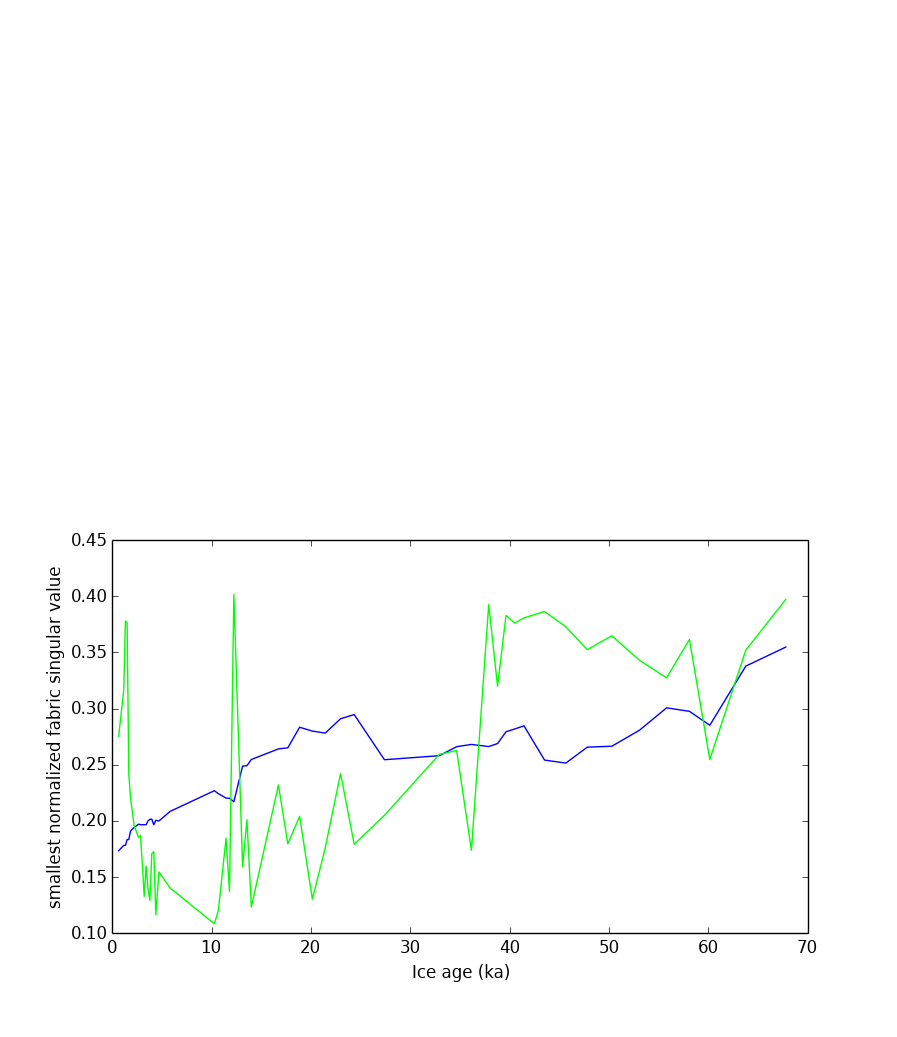
\includegraphics[width=12cm]{waisfit}
\end{figure}
\begin{figure}
\caption{Schmidt plot of girdle fabric produced under uniaxial compression. The grains rotate to the vertical axis. As they do, they are consumed by grains with lower strain energy.} 
\includegraphics[width=7cm]{girdle}
\end{figure}

The models fits the WAIS divide thin section fabric samples quite well. Jeffery's equation predicts grain rotation for a bulk strain rate well. Indeed, rotation via Jeffery's equation provides a better fit than using vorticity tensor derived for each grain individually. The transition from girdle to single maxima deeper in the core due to increased horizontal shear is captured resonably well, however the thin sections show a more diffuse single maximum developing. In these models, accumulation is assumed to be constant. Varying accumulation may contribute to spurious oscillations of the thinning function used to drive the model. In addition, grain boundary mobility for the model is held constant, which causes recrystallization of Pleistocene ice to be under-predicted.  

Future work will include coupling of the fabric model to a fully anisotropic flow model. This is necessary to investigate flow disruptions such as boudinage and folding. In addition, recent results \citep{montgomery-smith2011} show that coupled Stokes-Jefferys equations modeling fiber suspensions can induce intiial perturbations in the orientation distribution function to grow significantly in short amounts of time. The case of ice fabric is extremely similar. This opens up the possibility that small perturbations of the intitial fabric could grow into persistent large perturbations. This could be a source of the sometimes chaotic flow disturbances observed in some ice cores.


\bibliographystyle{agu}
\bibliography{anis}
\appendix
\section{Algorithm for the fabric model}

\textbf{Require:} Fabric c-axis orientations $\mathbf{c_i}$, grain radii $r_i$, bulk strain rate $D$, vorticity tensor  $W$, connectivity information $C_{ij}$;
\\
\textbf{For} each grain $\mathbf{g_i}$:
\\
\intent -Find local stress on each grain;
\\
\indent -Find areas of each boundary between grains;
\\
\textbf{For} each boundary of grain $\mathbf{g_i}$
\\
\indent -Find grain growth rate over each boundary due grain boundary energy, dislocation density, and impurity content;
\\
\textbf{End For}
\\
\indent -Add contributions to grain growth of the boundary with each neighbor. Integrate grain growth over each boundary over the timestep;
\\
\indent -Polygonize grain with probability $p$, depending on strain;
\\
\indent -Rotate grain by integrating Jeffery's equation through the timestep;
\\
\textbf{End For}
\\
-Advance time by $\delta t$
\\
-Return to \textbf{Start}.

\end{document}
